\chapter{Tendencias y Estado del arte}

Antes de adentrarnos de lleno en el análisis del problema y la realización de nuevas metodologías, es necesario estudiar y comprender el estado actual de esta temática en el estado del arte. Debido a que no se ha visto tan explotada como otros ámbitos de la IA, como es el caso de los modelos convolucionales o el aprendizaje automático supervisado tabular, podemos encontrar continuos cambios y nuevas vertientes que pueden inspirarnos a la hora de abordar el problema.

Hasta hace una década, buena parte de las técnicas diseñadas especialmente para series temporales y predicción a largo plazo, se basan principalmente en la descomposición las mismas en subcomponentes mucho más sencillas de procesar, las cuales pueden seguir un enfoque similar a divide y vencerás: descomponer la red en diferentes elementos, y mediante un mecanismo de agregación (aditivo, multiplicativo, o estadístico), recomponer la solución a la tarea. Sin embargo, se trata de una estrategia últimamente menos utilizada, en decadencia a favor de nuevas técnicas \\

Actualmente, una de las principales tendencias consiste en adaptar modelos originalmente desarrollados para otras modalidades. Un ejemplo de ello es el uso de convoluciones, ampliamente utilizadas en visión por computador, con el objetivo de capturar patrones locales en las secuencias y reducir la dimensionalidad del modelo. Previamente, también se han explorado arquitecturas recurrentes, como las Recurrent Neural Networks (RNN) y sus variantes más avanzadas, como las Long Short-Term Memory (LSTM) \cite{6795963}, aunque estas presentaban ciertas limitaciones en cuanto a capacidad de paralelización y en la modelización de relaciones temporales de mayor alcance, ya que para lograrlo aumentaba en exceso el tamaño de la red para incorporar más conexiones.\\

Más recientemente, ha ganado protagonismo la adaptación de mecanismos provenientes del procesamiento de lenguaje natural, en particular los Transformers, debido a su capacidad para modelar dependencias a largo plazo de forma eficiente. Además, comparten una motivación estructural con las series temporales: la necesidad de preservar una secuencia ordenada y coherente en la entrada, lo que permite aprovechar su arquitectura basada en atención para tareas de predicción.\\

A continuación, nos adentraremos de lleno en dichas propuestas, con el fin de aclarar, en primer, los conceptos clave acerca de las series temporales, y además, entender las problemáticas que surgen durante su procesado.

\section{Procesamiento básico de Series Temporales}

En la introducción, se han presentado brevemente las características fundamentales de las series temporales: su estructura temporal, caracterizada por muestreo, la importancia del orden de medición, y la necesidad de mantener las relaciones temporales para lograr aprender de forma efectiva.\\

Pero, en esta sección, profundizaremos en los aspectos clave del preprocesamiento necesario para su análisis de manera más formal, ya que a diferencia de otros tipos de datos, las series temporales requieren una atención especial a la dimensión temporal, y cualquier alteración en su estructura puede afectar directamente la capacidad del modelo para aprender los patrones subyacentes en ella. Por ello, es fundamental centrarnos en cuestiones como la frecuencia de muestreo, la consistencia temporal, el tratamiento de valores faltantes, y la normalización de las variables.

\subsection{Modelos basados en descomposición}

Las series temporales pueden exhibir una gran cantidad de patrones y comportamientos, los cuales son interesantes de estudiar y visualizar con claridad para estudiar que posible enfoque seguir a la hora de resolver el problema. Diferenciando cada una de las partes, podemos tratar de resolver cada una de ellas por separado, y posteriormente, construir un modelo agregado capaz de solucionar nuestro problema.\\

Frecuentemente, podemos encontrar 3 comportamientos, los cuales son fácilmente identificables incluso gráficamente, que nos permiten obtener información bastante valiosa acerca del problema que estamos estudiando, y nos facilitan la decisión de escoger la técnica adecuada:

\begin{itemize}
	\item \textbf{Tendencia}. Es el movimiento de los valores de serie a largo plazo, es decir, el comportamiento mostrado por los datos a la hora de estudiar su progresión desde el inicio de la serie hasta su final. El objetivo es encontrar si esta mantiene una dirección, de manera general, en su periodo de muestreo, buscando si sigue un comportamiento creciente, decreciente o constante, al igual que en el caso de estudio de monotonía clásico en funciones. Normalmente, se representan mediante comportamientos sencillos, y no se ven afectadas por grandes variaciones o el impacto de otras componentes de la serie, como variables aleatorias u otros factores externos. Normalmente, podemos modelarla haciendo uso de funciones elementales, como ecuaciones lineales o funciones exponenciales, logarítmicas o polinomiales.
			
	A veces, se requieren procesos de suavizado para así poder eliminar el efecto de otras componentes ruidosas que rodean la tendencia real de la serie. Esto se puede conseguir, de manera similar a la convolución, desplazando una ventana a lo largo de la serie, de manera que los valores dentro de ella sean suavizado. La forma más habitual de lograrlo es con una media móvil, la cual, cuanto mayor amplitud tenga, mayor reducción de ruido conseguiremos.
	
	En la figura \ref{trend}, podemos ver un ejemplo de su cálculo representado gráficamente sobre el dataset Air Passengers \cite{box1976time}.
	
	\begin{figure}[h] %con el [H] le obligamos a situar aquí la figura
		\centering
		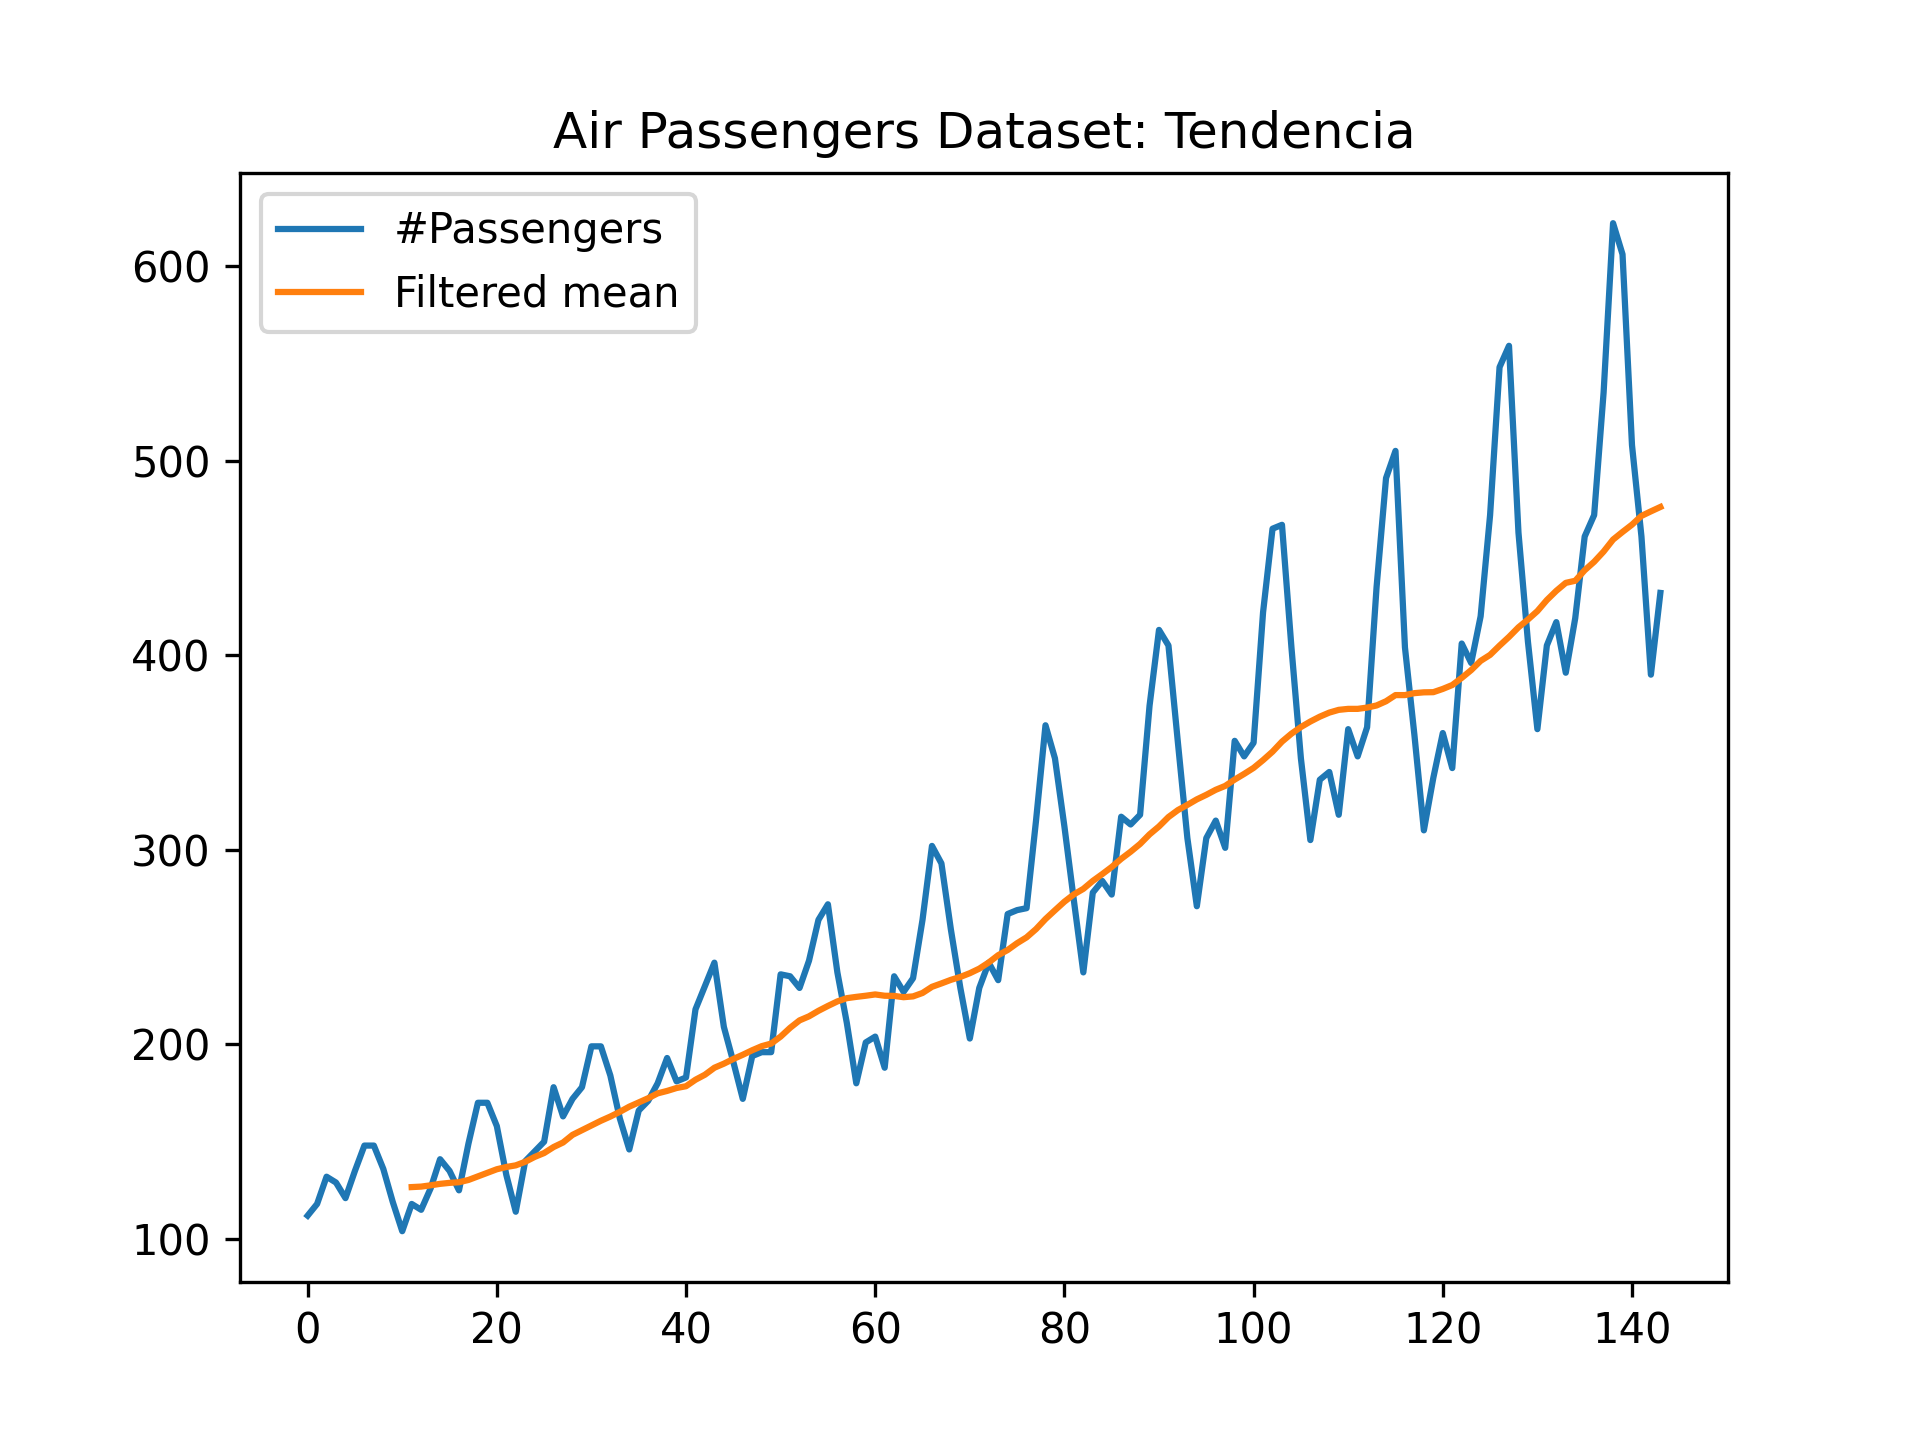
\includegraphics[scale=0.6]{img/trend}
		\caption{Estudio de la tendencia en el dataset Air Passengers}
		\label{trend}
	\end{figure}  	
	
	\item \textbf{Estacionalidad}. Son fluctuaciones periódicas y predecibles dentro de la serie temporal, las cuales siguen una determinada frecuencia y que pueden ser fácilmente modelables una vez se observa al menos un periodo. Normalmente, coinciden con unidades de medida de calendario, pudiendo encontrar así frecuecias semanales, mensuales, trimestrales, anuales... etc. Normalmente, son un factor visualmente sencillo de identificar, el cual apenas varía ente períodos, y que nos permite obtener información muy valiosa para el modelado.
	
	Podemos encontrar este comportamiento, por ejemplo, en los desplazamientos realizados durante las épocas vacionales: podremos observar un patrón de crecimiento en estas en Navidad y las vacaciones de verano, principalmente julio y agosto; y en el resto de meses el comportamiento será a la baja. Y eso ocurrirá con un período anual, ya que dichas fechas se ubican siempre en el mismo lugar. Diferente caso sería con Semana Santa, ya que su fecha no es coincidente todos los años y no cumple al 100\% de estacionalidad como las otras dos, ya que aunque es acotable en calendario, no es exactamente coincidente anualmente.
	
	En el caso del dataset anterior, se puede observar esta estacioalidad claramente (figura \ref{season})
	
		\begin{figure}[h] %con el [H] le obligamos a situar aquí la figura
		\centering
		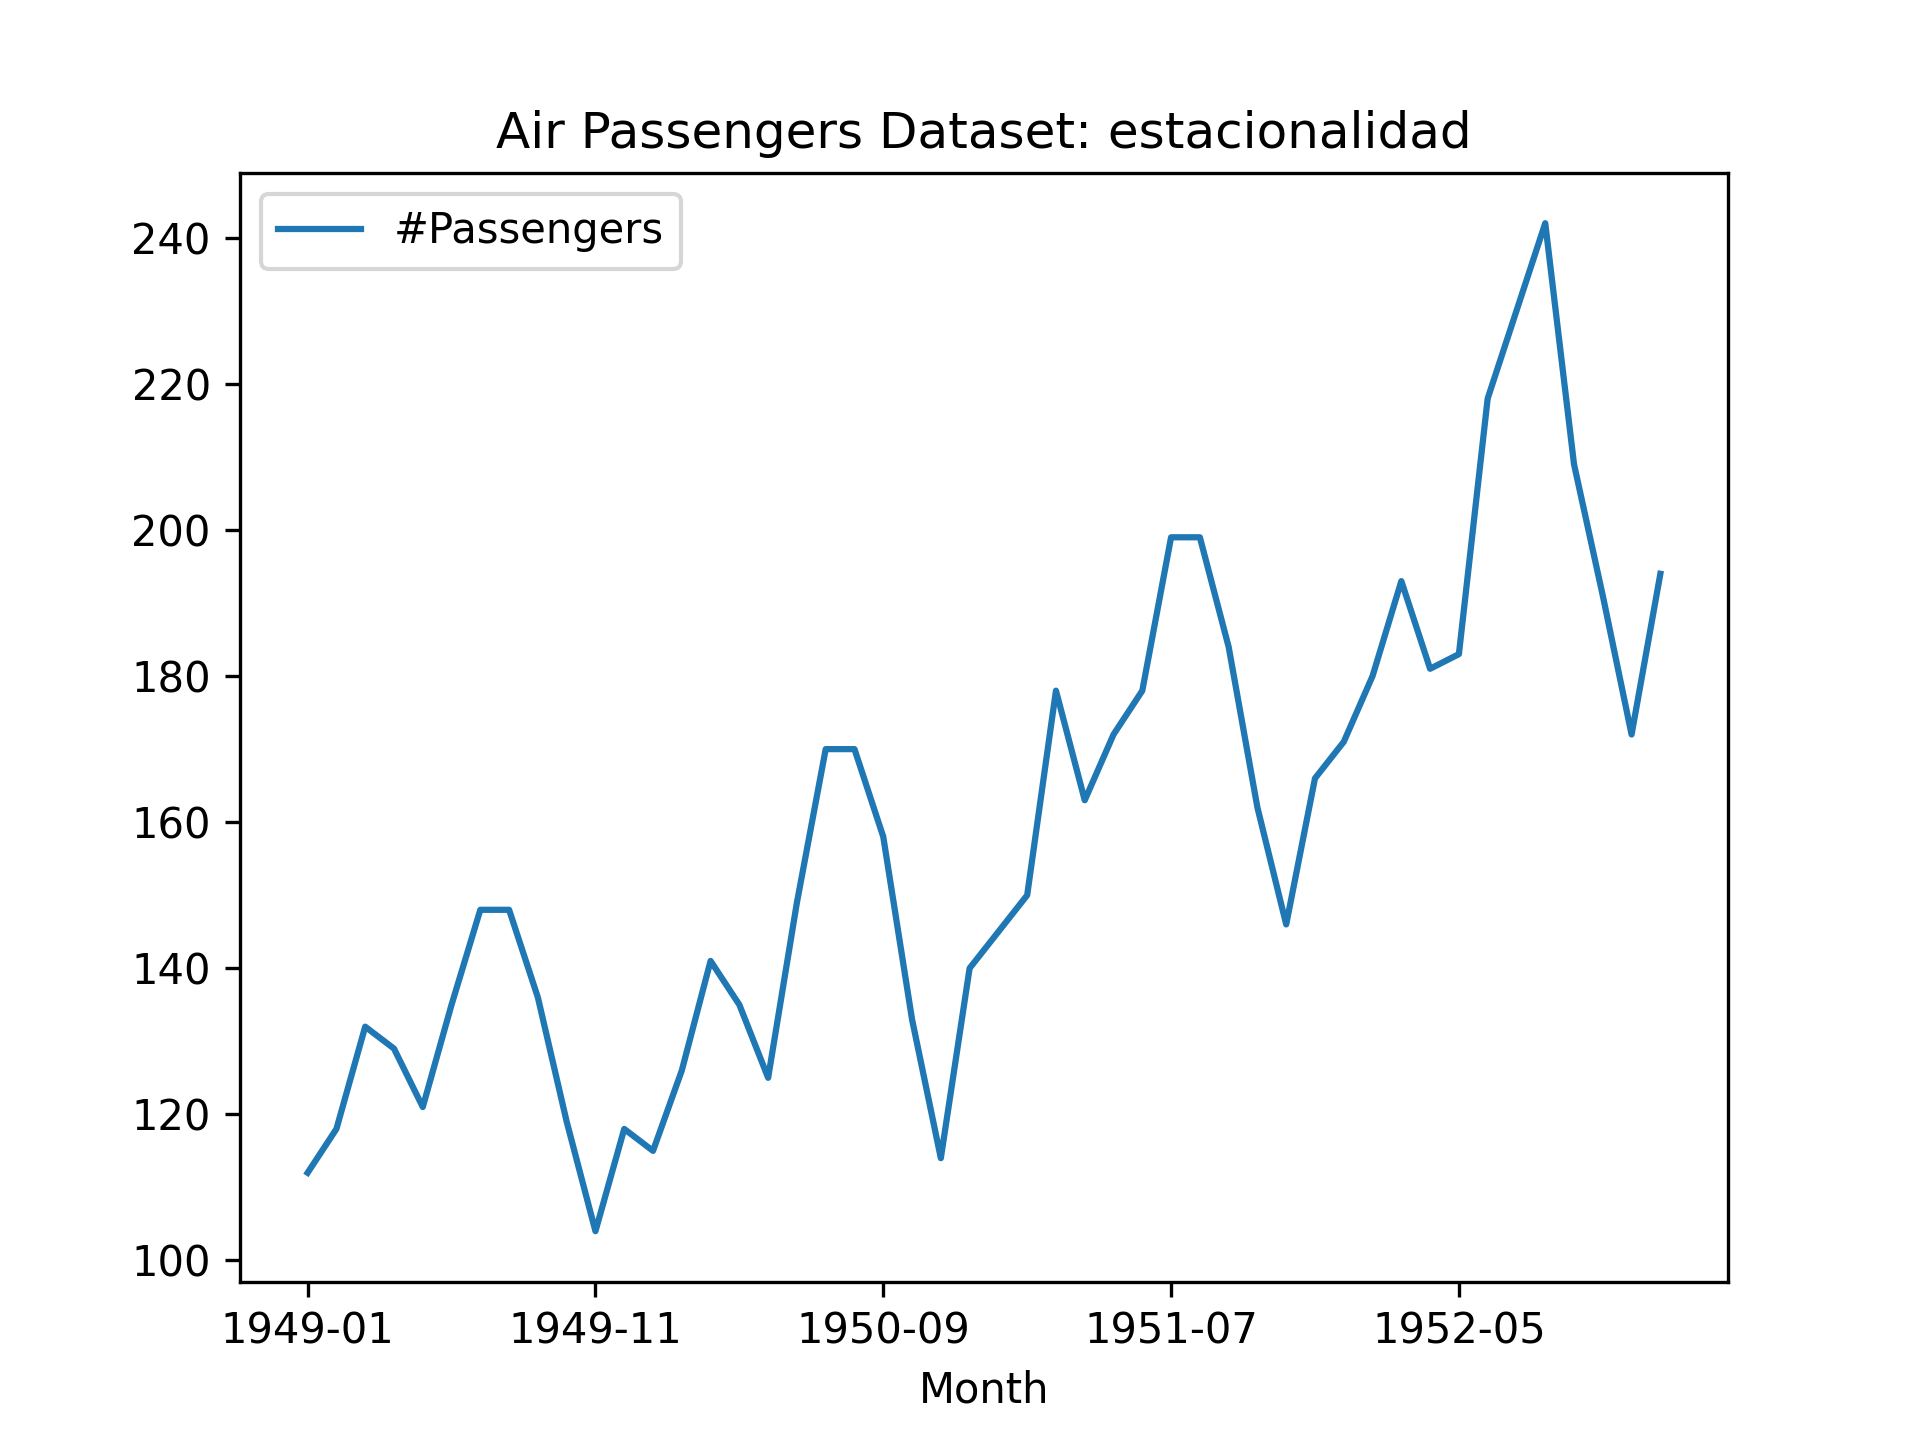
\includegraphics[scale=0.6]{img/season}
		\caption{Estudio de la estacionalidad en el dataset Air Passengers}
		\label{season}
	\end{figure}  	
	
	\item \textbf{Ciclo}. Son también fluctuaciones de la serie temporal, pero, a diferencia de ser regulares, siguen un período irregular de logitud fija. Normalmente, está vinculado a eventos que no están especialmente vinculados a fenómenos de calendario. El ejemplo más representativo podría ser la tendencia de crecimiento económico de un país, o el comportamiento de las acciones en bolsa de una sociedad anónima. 
	
	En la figura \ref{ciclo} podemos un ejemplo de este comportamiento con los permisos concedidos para la construcción de viviendas en EEUU \cite{techcharts2012housing}, donde no podemos encontrar patrones claros como en Air Passengers.
	
			\begin{figure}[H] %con el [H] le obligamos a situar aquí la figura
		\centering
		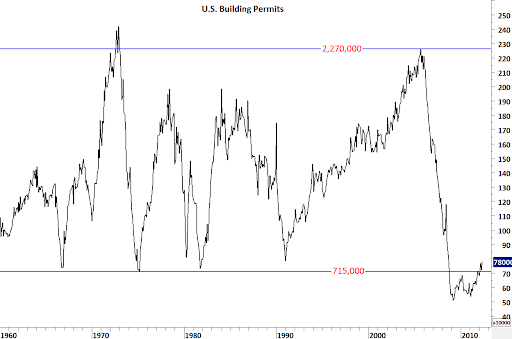
\includegraphics[scale=0.55]{img/ciclo}
		\caption{Estudio de ciclos en USA building permits}
		\label{ciclo}
	\end{figure}  	
	
\end{itemize}

Una vez comprendidos estos conceptos, podremos utilizar su información para decidir qué modelo se adapta mejor a nuestro problema y además tratar de modelar la tendencia y la estacionalidad. Anteriormente, mencionamos la gran utilidad de modelos como ARIMA, que funciona bajo este concepto. Pero no se trata del único modelo existente bajo este paradigma, sino uno de los más utilizados. En función del mecanismo de agregación de la solución, podemos clasificar las técnicas en dos grupos:

\begin{itemize}
	\item \textbf{Descomposición aditiva}. Realiza una separación de la serie temporal varias componentes, las cuales son modeladas por separado y sumadas entre si para dar lugar a la función predicha final (ecuación \ref{sum}). Es la más sencilla de usar en casos simples. Es indicada cuando las fluctuaciones estacionales por las variaciones entorno a la tendencia no varían con el valor de la serie temporal, es decir, pueden prácticamente mantenerse entre a lo largo de toda la serie sin apenas cambios. En general, se usa cuando los elementos no depende los unos de otros.
	
	\begin{equation}
	y(t) = T(t) + S(t) + C(t) + E(t)
	\label{sum}
	\end{equation}

	\item \textbf{Descomposición multiplicativa}. Se utiliza esta alternativa cuando las diferentes componentes dependen en nivel general de la serie (ecuación \ref{prod}). Es el caso de las series en las cuales los aumentos en la tendencia provocan aumentos también los picos de las tendencias estacionales o los ciclos.  Por ejemplo, en el dataset de Air Passengers, el comportamiento que se da es de este tipo.
	
	\begin{equation}
		y(t) = T(t) \times S(t) \times C(t) \times E(t)
		\label{prod}
	\end{equation}
	
\end{itemize}

Donde, en ambos casos:

\begin{itemize}
	\item \textit{T(t)}: Componente de la tendencia
	
	\item \textit{S(t)}: Componente estacional
	
	\item \textit{C(t)}: Componente cíclica
	
	\item \textit{E(t)}: Componente aleatoria y error
\end{itemize}

La elección de cada método depende, por tanto, de los datos, y nos beneficiaremos, como ya hemos visto a lo largo de la definición, de una adecuada visualización de los mismos cuando sea posible.

A continuación, definiremos en mayor detalle 3 de los algoritmos basados en descomposición más usados: STL \cite{cleveland1990stl}, ARIMA \cite{box1970time} y Prophet \cite{taylor2018prophet}.

\subsubsection{STL}

Esta técnica, llamada \textit{Seasonal Time-Series Decomposition}, nos permite descomponer la serie en partes más sencillas de modelar, separando la serie en tres componentes básicas: tendencia, estacionalidad y resto, siguiendo así el esquema visto anteriormente. De esta forma, podemos comprender en mayor detalle cómo evolucionan los valores a lo largo del tiempo, y comprender mejor cómo modelar su comportamiento. Para obtener un modelo para cada una de ellas,  normalmente se sigue un proceso de 3 pasos que nos permite aislar la información.

\begin{enumerate}
	\item \textbf{Extracción de la tendencia}. Se comienza extrayendo la tendencia de la serie para así obtener el comportamiento subyacente de la misma, y saber si es creciente, decreciente o se mantiene constante. En este algoritmo, se consigue mediante un proceso de suavizado, llamado \textit{Locally Estimated Scatterplot Smoothing} (Loess) de manera iterativa. Para ello, primero se comienza aplicando Loess, de manera que se suavizan los valores realizando una regresión no parámetrica, donde se observan los valores cercanos a cada timestamp de manera que se realiza un promedio que reduce las diferencias en el entorno. Si la serie es muy compleja o ruidosa, es posible que sea necesario repetir este proceso varias veces, por lo que se convierte en un proceso iterativo, utilizando tamaños mayores de ventana entorno a cada valor.
	
	Dicha ventana se estima a través de pesos, los cuales se ven reducidos cuanto más alejados al valor están. Estos se rigen por el valor de amplitud \textit{h}, que recogen las ecuaciones clásicas de la regresión de Loess. Dado un conjunto de datos \((t_i, y_i)\), el valor suavizado en \( t_0 \) se calcula como:
	
	\[
	\hat{y}(t_0) = \mathbf{x}_0^\top \hat{\boldsymbol{\beta}}(t_0)
	\]
	
	donde \(\hat{\boldsymbol{\beta}}(t_0)\) se obtiene minimizando la suma ponderada de errores:
	
	\[
	\hat{\boldsymbol{\beta}}(t_0) = \arg\min_{\boldsymbol{\beta}} \sum_{i=1}^n w_i(t_0) \left(y_i - \mathbf{x}_i^\top \boldsymbol{\beta}\right)^2
	\]
	
	Los pesos \( w_i(t_0) \) dependen de la distancia temporal y se definen, habitualmente, con el kernel tricúbico:
	
	\[
	w_i(t_0) = \left(1 - \left|\frac{t_i - t_0}{h}\right|^3\right)^3, \quad \text{para} \quad |t_i - t_0| < h
	\]
	
	El valor arrojado será 0 fuera del intervalo, y un valor entre 0 y 1 dentro de él, seleccionando así la relevancia de cada punto respecto a sus valores del entorno.
	
	\item  \textbf{Extracción de la estacionalidad}. Para extraer la estacionalidad, debemos aislarla de la tedencia que modelamos en el paso anterior. Para ello, basta con restar dicha componente a la serie original, y así disponer ahora únicamente del los patrones estacionales y el ruido. 
	$$y'(t) = y(t) - trend(t)$$
	
	A partir de aquí, debemos dividir la serie sin tendencia en subseries estacionales, agrupando los datos según la posición que ocupan dentro del ciclo; por ejemplo, si identificamos patrones con frecuencia mensual, se agruparían todos los valores correspondientes al mismo mes en años distintos, y sobre cada una de estas subseries se aplica un suavizado Loess de forma individual. Así, podremos capturar con precisión el patrón que se repite en cada estación, de manera similar a un promedio. Gracias a este proceso, podremos reconstruir una componente estacional coherente con las variaciones periódicas observadas en nuestro conjunto de datos, al que denominaremos \textit{s(t)}.
	
	\item \textbf{Obtención del resto}. Una vez extraídas tanto la tendencia como la estacionalidad, la componente residual se obtiene simplemente como la diferencia entre la serie original y la suma de las dos componentes anteriores:
	$$r(t) = y(t) - trend(t) - s(t)$$
	 Esta parte representa la variabilidad no explicada por los patrones sistemáticos de largo plazo ni por los ciclos periódicos, e incluye tanto el ruido aleatorio como cualquier información no capturada por el modelo. Si bien no es modelable, es muy útil para identificar si la serie es correctamente modelable por este método, ya que si observamos demasiada información en esta componente, nos está indicando que una parte importante de la información no está siendo recogida. Lo deseable es la que la varianza descrita sea la mínima posible. Sin embargo, hay algunos casos en los que encontrar puntos extremos es de utilidad, y se trata de la búsqueda de valores anómalos. Si la serie restante permanece estable y con poca varianza, a excepción de ciertos puntos, puede ser de interés estudiar qué ocurrió en dichos instantes, ya que su comportamiento se sale del comportamiento habitual modelado.
\end{enumerate}

En su publicación original, podemos encontrar un ejemplo de ejecución sobre el conjunto de datos \textit{Daily Carbon Dioxide Data} (ver figura \ref{stl}), que recoge información sobre las emisiones de $CO_2$ desde el 17 de abril de 1974 hasta el 31 de diciembre de 1986, y permite observar la información recogida por cada una de las componentes.

\begin{figure}[!htp] %con el [H] le obligamos a situar aquí la figura
	\centering
	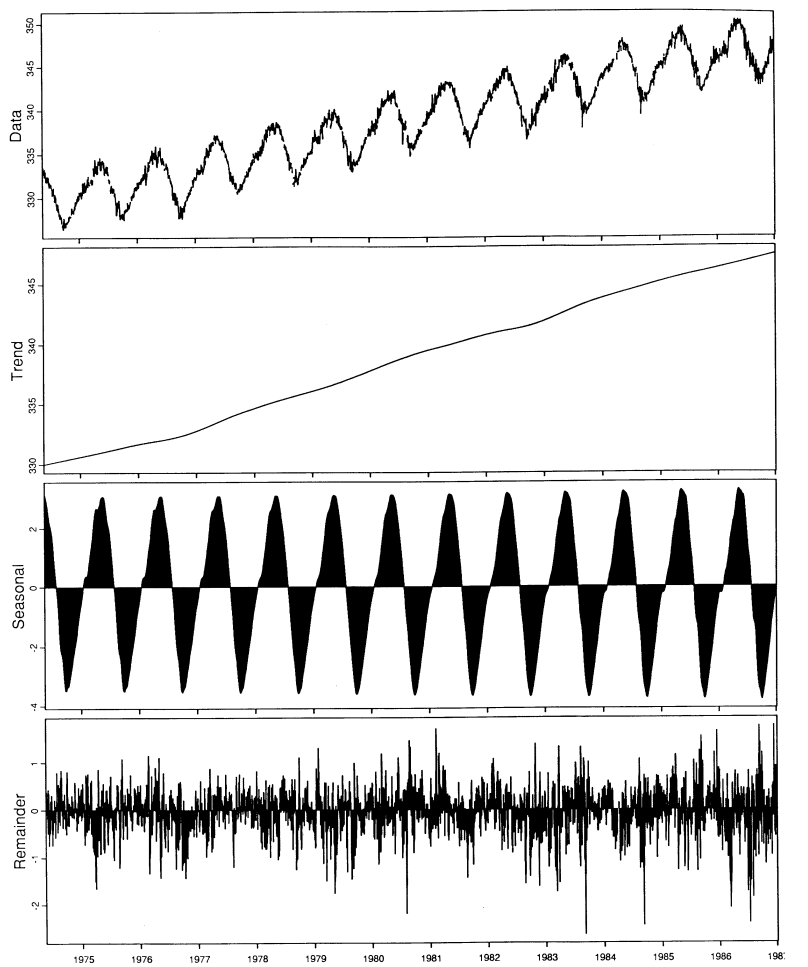
\includegraphics[scale=0.35]{img/stl}
	\caption{Ejemplo de caso de estudio empleando STL: Daily Carbon Dioxide Data \cite{cleveland1990stl}}
	\label{stl}
\end{figure}  	

En este caso, podemos apreciar visualmente una serie fácilmente modelable por este enfoque, ya que la curva describe una tendencia creciente bastante clara, y los periodos estacionales están bastante bien delimitados y no se ven influenciados por el crecimiento recogido en la tendencia. Es un ejemplo perfecto para el uso de los modelos basados en descomposición aditiva.\\

Sin embargo, esta forma de modelado presenta varias limitaciones, que acotan su funcionamiento a problemas simples:

\begin{itemize}
	\item Sólo se limita a descomponer series de naturaleza aditiva, por lo que aquellas en las que las diferentes componentes se vean influenciados entre sí requerirán técnicas propias de modelos multiplicativos.
	\item Pueden perderse gran cantidad de detalles explicados por los datos, debido a la configuración del parámetro de suavizado. Si alisamos de más la serie, podemos estar perdiendo información clave acerca de nuestro problema, dejando completamente de lado ciertos comportamientos sutiles, lo cual aumenta la tasa de error. Debemos escoger adecuadamente los valores al aplicar Loess.
	\item Es costoso computacionalmente en caso de series de larga duración, ya que el cálculo de aplicar el kernel se hace para cada punto en cada iteración sobre el conjunto de datos, tanto para encontrar la tendencia como para luego generalizar la estacionalidad.
\end{itemize}

Pero, sin lugar a dudas, la principal desventaja de este método es que no consigue por sí solo lo que deseamos resolver en este trabajo: predecir, sobre todo, a largo plazo. STL es un procedimiento muy útil que nos permite entender el comportamiento de los datos, y descomponerlo para comprender el funcionamiento de cada componente, pero no es posible por sí solo realizar predicciones. Dependemos del apoyo de otros procedimientos que nos permitan estimar , basándonos en este historial, la progresión de las componentes extraídas como la tendencia (modelable por regresión), y la estacional, la cual podría ser evaluada de manera simplificada por su valor medio histórico por intervalo.\\

Esto lo hace en un método interesante desde el punto de vista de análisis, y que permite dar lugar a modelos que sí son capaces de estimar predicciones futuras, pero no es una herramienta por sí sola que nos permita resolver la tarea que nos concierne en este trabajo.





\subsubsection{ARIMA}

Basándonos de nuevo en el método de descomposición de series, podemos encontrar el modelo \textbf{ARIMA} (\textit{AutoRegressive Integrated Moving Average}) una técnica estadística ampliamente utilizada para el modelado de series temporales univariantes. Como ya adelantamos en la introducción del proyecto, su estructura se basa en la combinación de tres componentes principales: una parte autoregresiva (AR), una parte integrada (I) y una parte de media móvil (MA). Cada una de estas partes permite capturar diferentes aspectos del comportamiento temporal de los datos.

\paragraph{Componente autoregresiva (AR)}
\mbox{}

Esta parte del modelo representa la relación entre el valor actual de la serie y sus valores pasados. Supone que el valor presente puede explicarse como una combinación lineal de observaciones anteriores, los cuales se denominan retardos o lags. Normalmente, el número de lags a emplear es un hiperparámetro clave del modelo, el cual es controlado por  \( p \).

	Matemáticamente, podemos expresarlo como:
	
	\[
	z_t = w_1 y_{t-1} + w_2 y_{t-2} + \cdots + wi_p y_{t-p} + \varepsilon_t
	\]
	
	donde:
	\begin{itemize}
		\item \( w_1, w_2, \ldots, w_p \) son los coeficientes autoregresivos que indican el peso o importancia de cada valor pasado. Cuando usamos el valor p, establecemos el número de valores con peso 1 que tomará nuestro modelo, mientras que el resto se mantienen a 0.  Pero, podríamos tener variantes en las que dichos pesos fueran valores flotantes entre 0 y 1 que permitan una ponderación más refinada de los valores.
		\item \( \varepsilon_t \) es el término asociado al error en el instante \( t \).
	\end{itemize}
	
	Gracias a la componente AR, podemos capturar relaciones de corto plazo y patrones de dependencia temporal, siempre que la serie sea estacionaria. Es habitual que muchas series temporales muestren este tipo de estructura, donde los valores pasados son predictivos del comportamiento futuro inmediato, como ya vimos con el caso de las temperaturas y el consumo eléctrico. Por tanto, la elección del parámetro \( p \) es clave:  un valor pequeño implica que sólo los valores más recientes tengan influencia, mientras que un valor mayor permite capturar relaciones más amplias en el tiempo, pero puede aumentar el riesgo de sobreajuste y se pierda localidad. En definitiva, se trata de un elemento esencial del rendimiento de ARIMA, por lo que es clave elegir adecuadamente su valor.

	\paragraph{Componente integrada (I)}
	\mbox{}
	
	
	La componente integrada del modelo ARIMA hace referencia al número de veces que es necesario integrar la serie temporal original para que esta se vuelva estacionaria, que es uno de los requisitos de este modelo.  De manera resumida, una serie estacionaria es aquella cuyas propiedades estadísticas, como la media, la varianza y la autocorrelación entre valores, se mantienen constantes a lo largo del tiempo,  como ya vimos en la definición de los modelos aditivos.\\
	
	La diferenciación nos permite eliminar tendencias o patrones sistemáticos de crecimiento o decrecimiento, facilitando el modelado de las componentes autoregresivas (AR) y de media móvil (MA). A pesar de que su nombre nos pueda insinuar un proceso complejo de integración analítica, al realizarse sobre valores numéricos, no es más que una diferencia de valores:
	
	\[
	y'_t = y_t - y_{t-1}
	\]
	
	Este proceso puede aplicarse tantas veces como sea necesario para lograr estacionariedad. Dicho número de repeticiones viene controlado por el valor de orden \( d \), que indica el número de veces que se ha diferenciado la serie. En general, el modelo ARIMA supone que tras aplicar \( d \) diferencias, la serie resultante \( y^{(d)} \) puede ser modelada por un proceso estacionario ARMA(\(p,q\)). Por tanto, el componente "I" de ARIMA es un procesamiento indispensable de la serie cuando no se cumpla el requisito de estacionariedad, y permitirá calcular sobre la serie resultante las componentes AR y MA con mayor facilidad. \\
	
\textbf{	AÑADIR FORMAS DE DETECTAR ESTACIONARIEDAD}
	
	\paragraph{Componente de media móvil (MA)}
	\mbox{}
	


\subsubsection{Prophet}

\subsection{RNN y LTSM}
\subsection{Transformers}

\section{Positional Encoding en Transformers}

\section{Conjuntos de datos disponibles}
